\subsection{Thermal sum}
\label{thermal sum}

When evaluating thermal integral, we will often encounter sums of the form
\begin{equation}
    \label{j func}
    j(\omega, \mu) = \frac{1}{2\beta} \sum_{\omega_n} 
    \ln\{\beta^2 [(\omega_n + i \mu) + \omega^2] \} + g(\beta),
\end{equation}
where the sum is over either the bosonic Matsubara frequencies $\omega_n = 2n \pi / \beta,\, n \in \mathbb{Z}$, or the fermionic ones, $\omega_n = (2n + 1) \pi /\beta ,\, n \in \mathbb{Z}$.
$\mu \in \R$ is the chemical potential.
$g$ may be a function of $\beta$, but we assume it is independent of $\omega$.
Thus, the factor $\beta^2$ could strictly be dropped, but it is kept to make the argument within the logarithm dimensionless.
We define the function
\begin{equation}
    \label{i func}
    i(\omega, \mu) = \frac{1}{\omega} \dv{\omega} j(\omega, \mu) 
    = \frac{1}{\beta} \sum_{\omega_n} \frac{1}{(\omega_n + i\mu)^2 + \omega^2}. 
\end{equation}

Assume $f(z)$ is an analytic function, except perhaps on a set of isolated poles $\{z_i\}$ located outside the real line. 
By exploiting the properties of $i n_B(i z)$, as described in \autoref{Conventions and notation}, we can rewrite the sum over Matsubara frequencies as a contour integral
\begin{equation*}
    \frac{1}{\beta} \sum_{\omega_n} f(\omega_n) 
    = \oint_\gamma \frac{\dd z}{2 \pi i} f(z) (i n_B(i z)),
\end{equation*}
where $\gamma$ is a contour that goes from $- \infty - i \epsilon$ to $+ \infty - i \epsilon$, crosses the real line at $\infty$, goes from $+ \infty - i \epsilon$ to $- \infty + i \epsilon$ before closing the curve.
The contour $\gamma$, and the change of integral contours is illustrated in \autoref{fig:integral contours}
This result exploits Cauchy's integral formula, by letting the poles of $in_B(iz)$ at the Matsubara frequencies ``pick out'' the necessary residues.
The integral over $\gamma$ is equivalent to two integrals along $\R \pm i \epsilon$,
\begin{align*}
    \frac{1}{\beta} \sum_{\omega_n} f(\omega_n) 
    &= \left(
        \int_{\infty + i \epsilon}^{-\infty + i \epsilon} \frac{\dd z}{2 \pi} 
        + \int_{-\infty - i \epsilon}^{\infty - i \epsilon}\frac{\dd z}{2 \pi}
    \right) 
    f(z) n_B(i z),
    \\
    & = \int_{-\infty - i \epsilon}^{\infty - i \epsilon}\frac{\dd z}{2 \pi}
    \left[
        f(z) + \left(f(z) + f(-z)\right) n_B(iz)
    \right].
\end{align*}
\begin{figure}
    \centering
    \begin{subfigure}{0.4\textwidth}
        \centering
        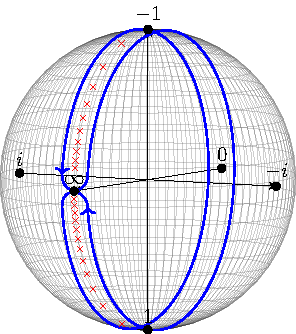
\includegraphics{thermal_field_theory/plots/integral_cont.pdf}        
    \end{subfigure}
    \begin{subfigure}{0.18\textwidth}
        \centering
        \begin{tikzpicture}
            \draw[-stealth] (0, 0) -- (1, 0);
        \end{tikzpicture}
        \end{subfigure}
    \begin{subfigure}{0.4\textwidth}
        \centering
        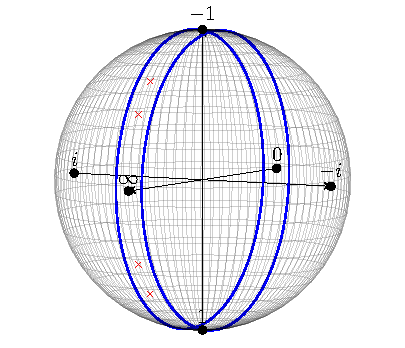
\includegraphics{thermal_field_theory/plots/integral_cont2.pdf}
    \end{subfigure} 
    \caption{The integral contour $\gamma$, and the result of deforming it into to contours close to the real line.}
    \label{fig:integral contours}
\end{figure}
In the last line, we have changed variables $z \rightarrow -z$ in the first integral, and exploited the property $n_B(-i z) = -1 - n_B(iz)$.
As $n_B(iz)$ is analytic on the real line, the result is the sum of residues of $f$ in the lower half plane.
The function
\begin{equation}
    f(z) = \frac{1}{(z + i \mu)^2 + \omega^2} 
    = \frac{i}{2 \omega } 
    \left(
        \frac{1}{z + i(\mu + \omega)} - \frac{1}{z + i(\mu - \omega)}
    \right)
\end{equation}
obeys the assumed properties, as it has poles at
$z = - i (\mu \pm \omega)$, with residue $1 / 2 \omega$, so the function defined in \autoref{i func} may be written \footnote{Assuming $\omega>\mu$.}
\begin{equation}
    i(\omega, \mu) 
    % = \left(\frac{-2 \pi i^2}{2 \pi \omega}\right)
    % [1 + n_B(\omega + \mu) + n_B(\omega - \mu)].
    = \frac{1}{2\omega}
    [1 + n_B(\omega + \mu) + n_B(\omega - \mu)].
\end{equation}

Using the anti-derivative of the Bose distribution, we get the final form of \autoref{j func}
\begin{equation}
    j(\omega, \mu) = \int \dd \omega'\, \omega' i(\omega', \mu)
    =  
    \frac{1}{2}\omega + \frac{1}{2\beta} 
    \left[
        \ln\left(1 - e^{-\beta(\omega + \mu)}\right)
        + \ln\left(1 - e^{-\beta(\omega - \mu)}\right)
    \right]
    + g'(\beta).
\end{equation}
The extra $\omega$-independent term $g'(\beta)$ is an integration constant.
(Noe om antipartikkel)

